\documentclass[conference]{IEEEtran}
\IEEEoverridecommandlockouts
% The preceding line is only needed to identify funding in the first footnote. If that is unneeded, please comment it out.
\usepackage{cite}
\usepackage{amsmath,amssymb,amsfonts}
\usepackage{algorithmic}
\usepackage{graphicx}
\usepackage{textcomp}
\usepackage{xcolor}
\def\BibTeX{{\rm B\kern-.05em{\sc i\kern-.025em b}\kern-.08em
    T\kern-.1667em\lower.7ex\hbox{E}\kern-.125emX}}
\begin{document}

\title{Evaluating the Impact of Interactivity on User Engagement in Virtual Reality Museums: A Comparative Study}\\

\author{\IEEEauthorblockN{1\textsuperscript{st}I Putu Bagus Gede Prasetyo\\Raharja}
\IEEEauthorblockA{\textit{Department of Informatics} \\
\textit{Institut Teknologi Sepuluh Nopember }\\
Surabaya, Indonesia \\
6025231010@student.its.ac.id}
\and
\IEEEauthorblockN{2\textsuperscript{nd}Muhammad Shafhi Kasyfillah}
\IEEEauthorblockA{\textit{Department of Informatics} \\
\textit{Institut Teknologi Sepuluh Nopember }\\
Surabaya, Indonesia \\
6025231053@student.its.ac.id}
\and
\IEEEauthorblockN{3\textsuperscript{rd}I Nyoman Gde Artadana\\Mahaputra Wardhiana}
\IEEEauthorblockA{\textit{Department of Informatics} \\
\textit{Institut Teknologi Sepuluh Nopember }\\
Surabaya, Indonesia \\
6025231022@student.its.ac.id}
\and
\IEEEauthorblockN{5\textsuperscript{th}Hadziq Fabroyir}
\IEEEauthorblockA{\textit{Department of Informatics} \\
\textit{Institut Teknologi Sepuluh Nopember }\\
Surabaya, Indonesia \\
Hadziq@its.ac.id}
}

\maketitle

\begin{abstract}
This document is a model and instructions for \LaTeX.
This and the IEEEtran.cls file define the components of your paper [title, text, heads, etc.]. *CRITICAL: Do Not Use Symbols, Special Characters, Footnotes, 
or Math in Paper Title or Abstract.
\end{abstract}

\begin{IEEEkeywords}
component, formatting, style, styling, insert
\end{IEEEkeywords}

\section{Introduction}
\IEEEPARstart{T}{he} integration of virtual reality (VR) technology in museums presents a significant opportunity to enhance user engagement, learning outcomes, and overall user experience. Previous research has shown that VR technology can enhance learning effectiveness and user experience by increasing perceived presence, immersion, realism, and satisfaction​. However, these outcomes can vary significantly based on the level of interactivity and the design of the VR interface.

This study aims to explore the effects of different levels of interactivity in VR museum exhibits on these variables, specifically focusing on Balinese traditional masks. Two VR museums will be created: one with static displays and plain sight explanations, and another with enhanced interactivity, including features such as holding the masks virtually and multimedia content like sound explanations.

By investigating these differences, this study aims to provide empirical evidence on the impact of VR interactivity in digital museums, contributing to the development of more effective and engaging VR educational tools. This research will utilize quantitative methods to measure engagement, comprehension, and usability, including time spent on tours, questionnaire scores, and System Usability Scale (SUS) scores. The findings will help in understanding how different VR designs can influence user experiences and learning outcomes, thereby supporting the hypothesis that increased interactivity enhances the effectiveness of VR museum exhibits.

\section{Related Works}
The integration of virtual reality (VR) into educational and museum settings has generated substantial academic interest. This section reviews key studies on the effectiveness of VR technology in enhancing user engagement, learning outcomes, and overall experience, with a particular focus on the role of interactivity. By examining these related works, the current study is contextualized within existing literature, highlighting the gaps it seeks to address.

Rahimi et al.~\cite{9286680} examine the impact of integrating virtual reality (VR) with physical exhibits in museums. Their research shows that VR-enhanced environments significantly boost learning and enjoyment compared to traditional and video-enhanced settings. By experimenting with different exhibit formats, the study provides valuable insights into how VR technology can create engaging and educational museum experiences, offering a promising direction for future hybrid museum spaces.

Kim et al.~\cite{6797425} discuss the development of an interactive VR interface for archaeological research and education. Focusing on the Northwest Palace of King Ashurnasirpal II in Iraq, the project integrates precise archaeological data into a VR environment, offering full-body immersion and user interaction with virtual artifacts. This VR museum aims to preserve and demonstrate cultural heritage, addressing the challenges of on-site conservation and providing a valuable tool for scholars and the public.

Despite these advancements, there remains a need for more empirical research on the specific effects of varying levels of interactivity in VR museum settings. Most existing studies focus broadly on the benefits of VR without isolating the impact of interactivity. This study aims to fill this gap by providing a comparative analysis of static versus interactive VR museum exhibits. By focusing on Balinese traditional masks, this research will offer unique insights into how interactivity influences user engagement, comprehension, and overall user experience in a cultural heritage context.

\section{Methodology}

This study employs a comparative design to evaluate the impact of interactivity on user engagement and system usability within virtual reality (VR) museum settings. The primary focus is on examining two distinct VR environments featuring Balinese traditional masks. The first environment, termed the "Non-Interactive VR Museum," presents the masks in a static display format with plain sight explanations, akin to traditional museum exhibits. Users in this setting can navigate through the museum but cannot interact with the masks beyond viewing them and reading the provided descriptions. The second environment, referred to as the "Interactive VR Museum," enhances user interaction by allowing users to virtually hold and manipulate the masks. This setting also includes multimedia content such as audio explanations that provide historical context, usage in cultural ceremonies, and associated myths. By comparing these two environments, the study aims to investigate how varying levels of interactivity influence user engagement, comprehension, retention of information, and overall system usability.

\begin{figure}[htbp]
    \centering
    \includegraphics[scale=0.8]{Report/src/bagan.png}
    \caption{Research Flow}
    \label{fig:researchflowchart}
\end{figure}



\subsection{Participants}
Participants for this study will be Balinese university students majoring in Information Technology, aged between 20 and 22 years. This demographic is specifically chosen due to their likely familiarity with digital technologies and potential prior exposure to VR environments, making them suitable candidates for the study. The selection criteria include their age and educational background to ensure a consistent baseline of digital literacy and technical knowledge.

\subsection{Variables}
The independent variable in this study is the type of VR museum exhibit. This variable has two levels:

\begin{itemize}
    \item Non-Interactive VR Museum: This setting presents the masks in a static display format with plain sight explanations.
    \item Interactive VR Museum: This setting enhances user interactivity with the exhibits, including features such as the ability to virtually hold and manipulate the masks, zoom in for detailed textures, rotate the masks for different views, and access multimedia content including audio explanations.
\end{itemize}

The study focuses on two primary dependent variables to measure the outcomes of the different VR settings:

\begin{itemize}
    \item User Engagement: Measured by the time participants spend on each museum tour. Longer times are interpreted as indicative of higher engagement, particularly if the time is spent interacting with the exhibits in the interactive VR museum.
    \item System Usability: Measured using the System Usability Scale (SUS), a 10-item questionnaire with responses ranging from "Strongly agree" to "Strongly disagree," resulting in a score from 0 to 100, with higher scores indicating better usability.
\end{itemize}

To ensure the consistency and validity of the results, several controlled variables will be maintained across both VR settings:

\begin{itemize}
    \item Content Consistency: The cultural and historical information provided about each mask will be identical in both settings to isolate the impact of interactivity.
    \item Navigation Experience: The navigation mechanics (e.g., movement through the museum space) will be consistent between the two settings to avoid confounding the results with differences in navigation ease or comfort.
    \item Participant Demographics: The study will target Balinese university students majoring in Information Technology, aged 20-22, to control for potential variations in background knowledge or familiarity with VR technology.
\end{itemize}

Confounding variables are factors other than the independent variable that might affect the dependent variable. Identifying and controlling for these variables is crucial to ensure the validity of the study's findings. In this study, potential confounding variables include:

\begin{itemize}
    \item Immersive Tendencies (ITQ Scores): Individual differences in immersive tendencies can influence how engaged participants are with the VR museum exhibits, regardless of the interactivity level. By measuring ITQ scores before the tours, these differences can be controlled for in the analysis to better isolate the effect of the VR museum type on engagement.
    \item Order of Joining: The sequence in which participants experience the interactive and non-interactive museums might influence their perceptions and engagement. For example, participants might be more engaged in the first experience due to novelty effects. Counterbalancing the order of joining and controlling for it in the analysis will help mitigate this potential confounding effect.
\end{itemize}
\subsection{Apparatus and Materials}
To conduct this study, the following apparatus and materials will be used:


\begin{itemize}
    \item VR Headsets: High-quality VR headsets such as the Oculus Rift or HTC Vive will be used to provide an immersive virtual reality experience for participants. These headsets will be used to display both the interactive and non-interactive VR museum settings.
    \item Computers: High-performance computers with the necessary specifications to run VR applications smoothly. These computers will ensure that the VR applications operate without technical issues that could affect the study's results.
    \item VR Controllers: Handheld VR controllers compatible with the VR headsets. These controllers will allow users to interact with the virtual objects, such as holding and rotating the masks in the interactive VR museum setting.
    \item Audio Equipment: High-quality headphones will be used to deliver immersive audio explanations and background sounds within the VR environments. This equipment will enhance the realism and engagement of the VR experience.
    \item Questionnaires: Digital versions of the Immersive Tendencies Questionnaire (ITQ) and System Usability Scale (SUS) questionnaires will be used to assess baseline immersive tendencies, usability, and other relevant metrics.
    \item Environment Setup: A quiet room with minimal distractions will be set up where participants can use the VR equipment comfortably. This controlled environment is necessary to ensure that external factors do not influence the participants' experience or the study's results.
\end{itemize}
\subsection{Procedure}
\subsubsection{Preparation}
\begin{itemize}
    \item Recruitment: Balinese university students majoring in Information Technology will be recruited for the study. Recruitment will be done through university channels, including announcements in classes, flyers, and emails.
    \item Briefing: Participants will receive a detailed overview of the study, including its purpose, what participation involves, the procedures to be followed, and any potential risks and benefits.
    \item Consent: Informed consent will be obtained from all participants. Participants will be informed about their rights, including the right to withdraw from the study at any time without penalty.
\end{itemize}
\subsubsection{Baseline Measurement}
\begin{itemize}
    \item ITQ Administration: Before the experiment sessions, participants will complete the Immersive Tendencies Questionnaire (ITQ) to assess their baseline immersive tendencies. This will help control for individual differences in how easily participants become immersed in virtual environments.
\end{itemize}
\subsubsection{Experiment Sessions}
\begin{itemize}
    \item Session Assignment: Participants will be randomly assigned to experience either the non-interactive or interactive VR museum first to counterbalance the order of exposure and control for potential novelty effects.
    \item Non-Interactive VR Museum: Participants assigned to this condition will explore the static VR museum with plain sight explanations. The time spent on the tour will be recorded to measure engagement.
    \item Interactive VR Museum: Participants assigned to this condition will interact with the VR museum using features like zooming, rotating masks, and accessing multimedia content. The time spent on the tour will be recorded to measure engagement.
\end{itemize}
\subsubsection{Post-Tour Assessment}
\begin{itemize}
    \item Post-Tour Questionnaire: After each tour, participants will complete a questionnaire designed to assess their understanding and retention of information about the masks.
    \item SUS Administration: Participants will also complete the System Usability Scale (SUS) to evaluate usability.
\end{itemize}
\subsubsection{Debriefing}
\begin{itemize}
    \item Debriefing Session: A debriefing session will be conducted to explain the study's purpose, answer any questions participants might have, and provide additional information about the research.
    \item Feedback Collection: Participants will be asked to provide feedback about their experiences in both VR museum settings. This feedback will be valuable for qualitative insights into the user experience.
\end{itemize}
\subsubsection{Data Analysis}
\begin{itemize}
    \item Data Compilation: Data from ITQ, time spent on tours, post-tour questionnaires, and SUS scores will be compiled for analysis.
    \item Descriptive Statistics: Calculate mean, standard deviation, median, and interquartile range (IQR) for each dependent variable in both groups.
\end{itemize}
\subsection{ANCOVA}

To evaluate the impact of the type of VR museum setting on user engagement, an Analysis of Covariance (ANCOVA) will be performed. The formula for ANCOVA is as follows:

\[ Y_{ij} = \mu + \tau_i + \beta(X_{ij} - \overline{X}) + \epsilon_{ij} \]

where:
\begin{itemize}
    \item \( Y_{ij} \) is the dependent variable for the \( j \)-th observation in the \( i \)-th group.
    \item \( \mu \) is the overall mean.
    \item \( \tau_i \) is the effect of the \( i \)-th group.
    \item \( \beta \) is the regression coefficient.
    \item \( X_{ij} \) is the covariate for the \( j \)-th observation in the \( i \)-th group.
    \item \( \overline{X} \) is the overall mean of the covariate.
    \item \( \epsilon_{ij} \) is the error term for the \( j \)-th observation in the \( i \)-th group.
\end{itemize}

\subsection{Wilcoxon}
To compare the usability scores between the non-interactive and interactive VR museum settings, the Wilcoxon signed-rank test will be used. The test statistic \( \ W \) is calculated as follows:

\[
W = \sum_{i=1}^n R_i^+
\]

where:
\begin{itemize}
    \item \( W \) is the test statistic.
    \item \( n \) is the number of paired samples.
    \item \( R_i^+ \) is the rank of the positive differences.
\end{itemize}

\subsection{Interpretation of Results} 
Interpret the results in the context of the study's hypotheses. The null hypothesis (H0) states that there is no significant difference in user engagement between the non-interactive and interactive VR museum settings after controlling for covariates. The alternative hypothesis (H1) states that there is a significant difference.

\begin{itemize}
    \item For ANCOVA: Evaluate the F-statistic and p-value to determine if there is a significant difference in user engagement after controlling for covariates.
\item For the Wilcoxon signed-rank test: Compare the test statistic to the critical value and p-value to determine if there is a significant difference in usability scores.
\end{itemize}
If the p-value is less than the significance level (typically 0.05), reject the null hypothesis in favor of the alternative hypothesis, indicating a significant difference between the groups.
\section{Result and Discussion}

\section{Conclusion}
% Before you begin to format your paper, first write and save the content as a 
% separate text file. Complete all content and organizational editing before 
% formatting. Please note sections \ref{AA}--\ref{SCM} below for more information on 
% proofreading, spelling and grammar.

% Keep your text and graphic files separate until after the text has been 
% formatted and styled. Do not number text heads---{\LaTeX} will do that 
% for you.

% \subsection{Abbreviations and Acronyms}\label{AA}
% Define abbreviations and acronyms the first time they are used in the text, 
% even after they have been defined in the abstract. Abbreviations such as 
% IEEE, SI, MKS, CGS, ac, dc, and rms do not have to be defined. Do not use 
% abbreviations in the title or heads unless they are unavoidable.

% \subsection{Units}
% \begin{itemize}
% \item Use either SI (MKS) or CGS as primary units. (SI units are encouraged.) English units may be used as secondary units (in parentheses). An exception would be the use of English units as identifiers in trade, such as ``3.5-inch disk drive''.
% \item Avoid combining SI and CGS units, such as current in amperes and magnetic field in oersteds. This often leads to confusion because equations do not balance dimensionally. If you must use mixed units, clearly state the units for each quantity that you use in an equation.
% \item Do not mix complete spellings and abbreviations of units: ``Wb/m\textsuperscript{2}'' or ``webers per square meter'', not ``webers/m\textsuperscript{2}''. Spell out units when they appear in text: ``. . . a few henries'', not ``. . . a few H''.
% \item Use a zero before decimal points: ``0.25'', not ``.25''. Use ``cm\textsuperscript{3}'', not ``cc''.)
% \end{itemize}

% \subsection{Equations}
% Number equations consecutively. To make your 
% equations more compact, you may use the solidus (~/~), the exp function, or 
% appropriate exponents. Italicize Roman symbols for quantities and variables, 
% but not Greek symbols. Use a long dash rather than a hyphen for a minus 
% sign. Punctuate equations with commas or periods when they are part of a 
% sentence, as in:
% \begin{equation}
% a+b=\gamma\label{eq}
% \end{equation}

% Be sure that the 
% symbols in your equation have been defined before or immediately following 
% the equation. Use ``\eqref{eq}'', not ``Eq.~\eqref{eq}'' or ``equation \eqref{eq}'', except at 
% the beginning of a sentence: ``Equation \eqref{eq} is . . .''

% \subsection{\LaTeX-Specific Advice}

% Please use ``soft'' (e.g., \verb|\eqref{Eq}|) cross references instead
% of ``hard'' references (e.g., \verb|(1)|). That will make it possible
% to combine sections, add equations, or change the order of figures or
% citations without having to go through the file line by line.

% Please don't use the \verb|{eqnarray}| equation environment. Use
% \verb|{align}| or \verb|{IEEEeqnarray}| instead. The \verb|{eqnarray}|
% environment leaves unsightly spaces around relation symbols.

% Please note that the \verb|{subequations}| environment in {\LaTeX}
% will increment the main equation counter even when there are no
% equation numbers displayed. If you forget that, you might write an
% article in which the equation numbers skip from (17) to (20), causing
% the copy editors to wonder if you've discovered a new method of
% counting.

% {\BibTeX} does not work by magic. It doesn't get the bibliographic
% data from thin air but from .bib files. If you use {\BibTeX} to produce a
% bibliography you must send the .bib files. 

% {\LaTeX} can't read your mind. If you assign the same label to a
% subsubsection and a table, you might find that Table I has been cross
% referenced as Table IV-B3. 

% {\LaTeX} does not have precognitive abilities. If you put a
% \verb|\label| command before the command that updates the counter it's
% supposed to be using, the label will pick up the last counter to be
% cross referenced instead. In particular, a \verb|\label| command
% should not go before the caption of a figure or a table.

% Do not use \verb|\nonumber| inside the \verb|{array}| environment. It
% will not stop equation numbers inside \verb|{array}| (there won't be
% any anyway) and it might stop a wanted equation number in the
% surrounding equation.

% \subsection{Some Common Mistakes}\label{SCM}
% \begin{itemize}
% \item The word ``data'' is plural, not singular.
% \item The subscript for the permeability of vacuum $\mu_{0}$, and other common scientific constants, is zero with subscript formatting, not a lowercase letter ``o''.
% \item In American English, commas, semicolons, periods, question and exclamation marks are located within quotation marks only when a complete thought or name is cited, such as a title or full quotation. When quotation marks are used, instead of a bold or italic typeface, to highlight a word or phrase, punctuation should appear outside of the quotation marks. A parenthetical phrase or statement at the end of a sentence is punctuated outside of the closing parenthesis (like this). (A parenthetical sentence is punctuated within the parentheses.)
% \item A graph within a graph is an ``inset'', not an ``insert''. The word alternatively is preferred to the word ``alternately'' (unless you really mean something that alternates).
% \item Do not use the word ``essentially'' to mean ``approximately'' or ``effectively''.
% \item In your paper title, if the words ``that uses'' can accurately replace the word ``using'', capitalize the ``u''; if not, keep using lower-cased.
% \item Be aware of the different meanings of the homophones ``affect'' and ``effect'', ``complement'' and ``compliment'', ``discreet'' and ``discrete'', ``principal'' and ``principle''.
% \item Do not confuse ``imply'' and ``infer''.
% \item The prefix ``non'' is not a word; it should be joined to the word it modifies, usually without a hyphen.
% \item There is no period after the ``et'' in the Latin abbreviation ``et al.''.
% \item The abbreviation ``i.e.'' means ``that is'', and the abbreviation ``e.g.'' means ``for example''.
% \end{itemize}
% An excellent style manual for science writers is \cite{b7}.

% \subsection{Authors and Affiliations}
% \textbf{The class file is designed for, but not limited to, six authors.} A 
% minimum of one author is required for all conference articles. Author names 
% should be listed starting from left to right and then moving down to the 
% next line. This is the author sequence that will be used in future citations 
% and by indexing services. Names should not be listed in columns nor group by 
% affiliation. Please keep your affiliations as succinct as possible (for 
% example, do not differentiate among departments of the same organization).

% \subsection{Identify the Headings}
% Headings, or heads, are organizational devices that guide the reader through 
% your paper. There are two types: component heads and text heads.

% Component heads identify the different components of your paper and are not 
% topically subordinate to each other. Examples include Acknowledgments and 
% References and, for these, the correct style to use is ``Heading 5''. Use 
% ``figure caption'' for your Figure captions, and ``table head'' for your 
% table title. Run-in heads, such as ``Abstract'', will require you to apply a 
% style (in this case, italic) in addition to the style provided by the drop 
% down menu to differentiate the head from the text.

% Text heads organize the topics on a relational, hierarchical basis. For 
% example, the paper title is the primary text head because all subsequent 
% material relates and elaborates on this one topic. If there are two or more 
% sub-topics, the next level head (uppercase Roman numerals) should be used 
% and, conversely, if there are not at least two sub-topics, then no subheads 
% should be introduced.

% \subsection{Figures and Tables}
% \paragraph{Positioning Figures and Tables} Place figures and tables at the top and 
% bottom of columns. Avoid placing them in the middle of columns. Large 
% figures and tables may span across both columns. Figure captions should be 
% below the figures; table heads should appear above the tables. Insert 
% figures and tables after they are cited in the text. Use the abbreviation 
% ``Fig.~\ref{fig}'', even at the beginning of a sentence.

% \begin{table}[htbp]
% \caption{Table Type Styles}
% \begin{center}
% \begin{tabular}{|c|c|c|c|}
% \hline
% \textbf{Table}&\multicolumn{3}{|c|}{\textbf{Table Column Head}} \\
% \cline{2-4} 
% \textbf{Head} & \textbf{\textit{Table column subhead}}& \textbf{\textit{Subhead}}& \textbf{\textit{Subhead}} \\
% \hline
% copy& More table copy$^{\mathrm{a}}$& &  \\
% \hline
% \multicolumn{4}{l}{$^{\mathrm{a}}$Sample of a Table footnote.}
% \end{tabular}
% \label{tab1}
% \end{center}
% \end{table}

% \begin{figure}[htbp]
% \centerline{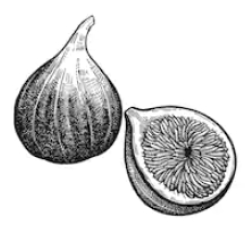
\includegraphics{fig1.png}}
% \caption{Example of a figure caption.}
% \label{fig}
% \end{figure}

% Figure Labels: Use 8 point Times New Roman for Figure labels. Use words 
% rather than symbols or abbreviations when writing Figure axis labels to 
% avoid confusing the reader. As an example, write the quantity 
% ``Magnetization'', or ``Magnetization, M'', not just ``M''. If including 
% units in the label, present them within parentheses. Do not label axes only 
% with units. In the example, write ``Magnetization (A/m)'' or ``Magnetization 
% \{A[m(1)]\}'', not just ``A/m''. Do not label axes with a ratio of 
% quantities and units. For example, write ``Temperature (K)'', not 
% ``Temperature/K''.

\section*{Acknowledgment}

The preferred spelling of the word ``acknowledgment'' in America is without 
an ``e'' after the ``g''. Avoid the stilted expression ``one of us (R. B. 
G.) thanks $\ldots$''. Instead, try ``R. B. G. thanks$\ldots$''. Put sponsor 
acknowledgments in the unnumbered footnote on the first page.

\bibliographystyle{IEEEtran}
\bibliography{references}


\end{document}
